\documentclass[conference,10pt]{IEEEtran}

\usepackage{cite}
\usepackage{amsmath,amssymb}
\usepackage{graphicx}
\usepackage{tabularx}
\usepackage{placeins}
\usepackage{balance}
\usepackage{algorithm}
\usepackage{algpseudocode}
\usepackage[hidelinks]{hyperref}

% Keep figure descriptions in the source for future accessible output.
\newcommand{\Description}[1]{}
\setlength{\emergencystretch}{1em}


\title{Thermal-Aware NoC Reconfiguration for Concurrent General-Purpose Computing and MoE Inference in 3D-Stacked Systems}
\author{Anonymous Author(s)}

\begin{document}


\maketitle

\begin{abstract}
An asynchronous agent can run general-purpose tasks alongside AI inference. We focus on AI inference with mixture-of-experts (MoE) models. In a 3D DRAM-stacked system, MoE dispatch traffic can contend with general-purpose memory requests at shared network-on-chip (NoC) outputs, delaying a step that needs both results. We place coherence traffic on a separate Mesh and reconfigure MoE paths using predicted demand. Configurable switches provide additional MoE channels and bypass intermediate routers. Before updating routes, the controller estimates completion time, accounting for network interface delays, memory bank access, and reconfiguration overhead. Operator-level dynamic voltage and frequency scaling and thermal-aware task scheduling manage execution under peak-temperature constraints.
\end{abstract}

\begin{IEEEkeywords}
hybrid bonding, 3D integration, mixture-of-experts, network-on-chip,
reconfigurable interconnect, memory-bank contention, thermal management
\end{IEEEkeywords}
\raggedbottom

\section{Introduction}
\label{sec:introduction}

An asynchronous agent can run general-purpose tasks alongside AI inference.
A later step that needs both results must wait for both branches. In 3D
DRAM-stacked systems, high-bandwidth links connect the logic and memory
dies~\cite{li2026helios}, while the network-on-chip (NoC) carries token
exchanges between nodes hosting different experts in a mixture-of-experts
(MoE) model. General-purpose traffic and MoE dispatch bursts can contend for
the same router output. Frequent short memory requests can add substantial
load, and queueing can delay responses needed by the agent.

MoE token exchange can involve many nodes in a single batch. Uneven expert
activation can concentrate traffic on a few node pairs and saturate even
short paths, while distant transfers consume forwarding capacity across
multiple routers. The communicating nodes and heavily used paths change with
inputs, model layers, and the dispatch and combine phases. Thermal coupling
between the stacked logic and DRAM tiers can also trigger throttling and
prolong inference.

RHT\_NoC dynamically combines horizontal and vertical torus loops according
to aggregate inter-ring traffic~\cite{xu2025rhtnoc}. Flows on the same combined
loop share its capacity. As heavily loaded node pairs change, finer-grained
connections can add bandwidth between neighboring nodes and bypass
intermediate routers for distant transfers.

We separate coherence traffic onto a dedicated Mesh and add configurable
switches to the MoE Mesh. The switch connections change with communication
demand. A predictor estimates
per-phase demand, and a configuration algorithm assigns packets to compatible
circuits under switch-conflict and network interface and memory bank capacity
constraints. The controller checks estimated completion time and
reconfiguration overhead before applying an update. Operator-level
energy-aware DVFS and thermal-aware task scheduling support execution under
peak-temperature constraints.

This work makes three contributions:
\begin{enumerate}
  \item We design a reconfigurable NoC for concurrent general-purpose
  workloads and MoE inference in 3D DRAM-stacked systems. Separate Mesh
  planes carry coherence and MoE traffic. The switch fabric
  provides local channels and cross-region paths that can be reassigned to
  individual node pairs between communication phases.

  \item We develop a phase-dependent method that predicts demand, selects
  compatible circuits, and assigns packets within shared network interface
  and memory bank capacities. A completion-time check accounts for
  reconfiguration overhead.

  \item We evaluate how the design affects the modeled readiness of a step
  that waits for both the general-purpose and MoE branches. The reduction in
  time to readiness relative to the baseline is XX\%.
\end{enumerate}

\setlength{\textfloatsep}{12pt}
\setlength{\floatsep}{10pt}

\section{Motivation}
\label{sec:motivation}

\subsection{Target System and Workloads}
\label{sec:target-system-workloads}

\begin{figure}[!tbp]
  \centering
  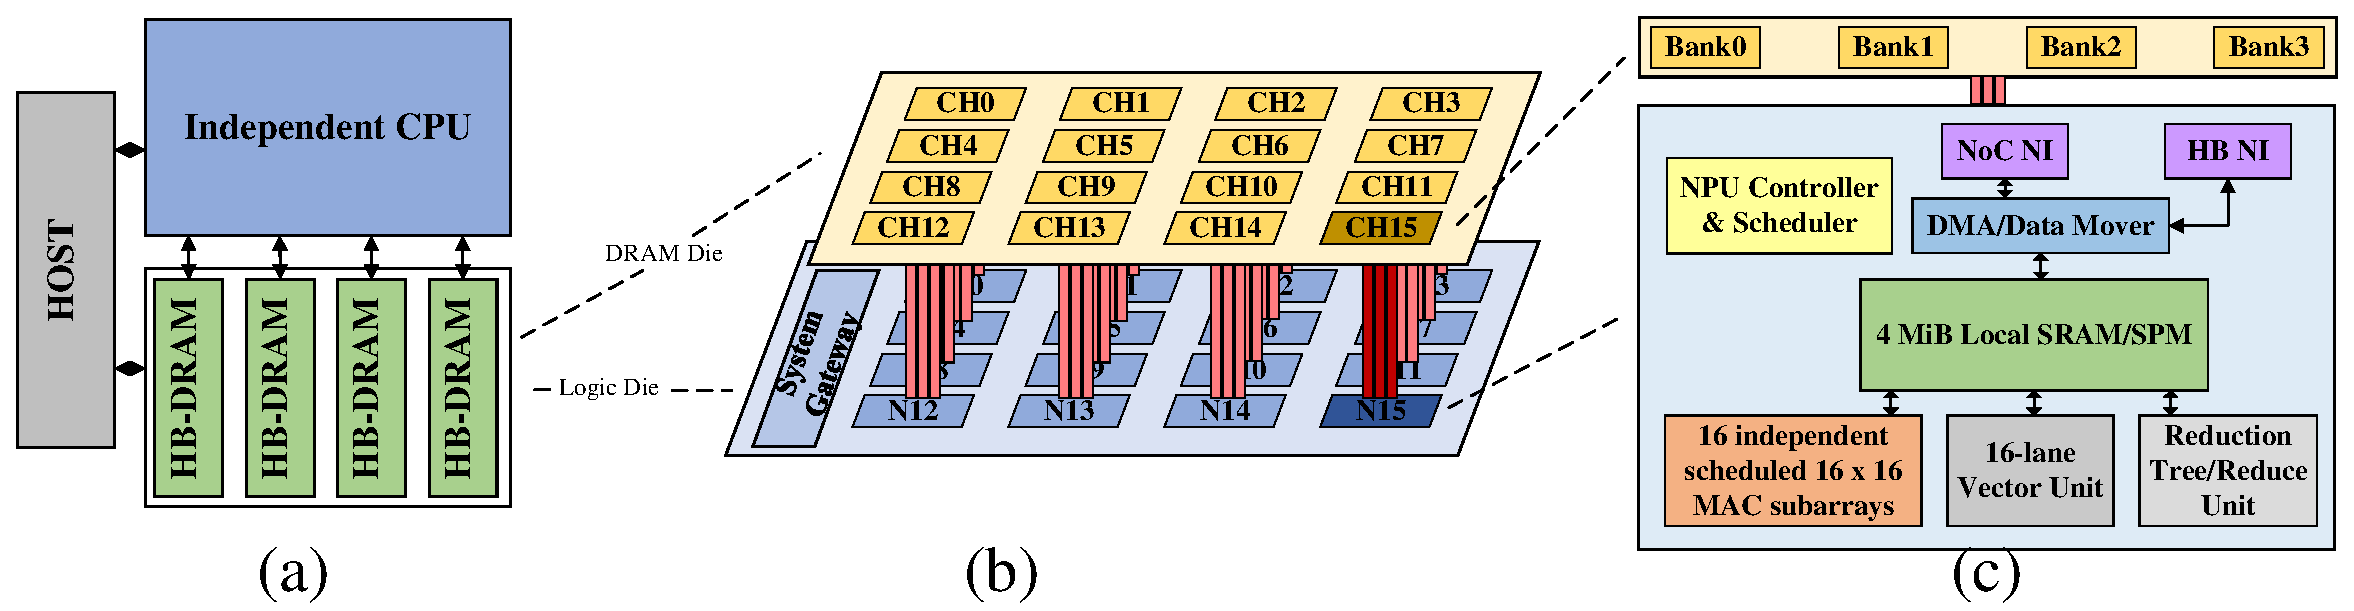
\includegraphics[width=\columnwidth]{figures/target_architecture_uniform_titles.pdf}
  \caption{Target 3D system. (a) Host and HB-DRAM organization. (b) Face-to-face
  integration of the $4\times4$ Logic-tier NPU mesh and the aligned DRAM
  channels. (c) Microarchitecture of an NPU--memory pair.}
  \Description{Three panels show the host and HB-DRAM organization, the
  vertically aligned NPU clusters and DRAM channels, and the internal
  organization of one NPU--memory pair.}
  \label{fig:target-architecture}
\end{figure}

Figure~\ref{fig:target-architecture} shows a 3D accelerator in which the
logic and memory tiers are integrated by face-to-face hybrid bonding.
Each NPU cluster in the logic tier is vertically aligned with a DRAM
partition and accesses it through a local hybrid-bond link. A baseline
horizontal $4\times4$ Mesh NoC connects the NPU clusters and carries
inter-cluster transfers, including MoE Dispatch and Combine traffic.
Local memory accesses and inter-cluster transfers therefore use distinct
physical paths. The stacked logic and DRAM dies are thermally coupled,
imposing a peak-temperature constraint on execution.

To study co-execution, we replay an MoE dispatch trace alongside synthetic
cache-coherence read requests that represent general-purpose memory traffic.
On the baseline, requests and responses share the horizontal Mesh with
MoE traffic.

The main MoE evaluation covers Qwen3-30B-A3B~\cite{qwen3report} and
Qwen1.5-MoE-A2.7B~\cite{qwen15moe} for language-model inference,
mini-SWE-agent~\cite{minisweagent} with a Qwen3-30B-A3B backend for
SWE-bench Lite tasks~\cite{swebench}, and LingBot TI2V~\cite{lingbotvideo}
for video generation. The auxiliary thermal scenario combines
WHISPER~\cite{whisper}, an ORB-SLAM3-derived SLAM workload~\cite{orbslam3},
and $\pi_{0.5}$~\cite{pi05}.


\subsection{Phase-Dependent Congestion in MoE Communication}

\noindent\textbf{Problem.}
HiBand adapts communication locality by switching among four topologies---
Full-Local, Local-Biased, Global-Biased, and Full-Global---that repartition
bandwidth according to broad communication locality~\cite{wang2026hiband}.
MoE communication can concentrate transfers around a small set of busy NPU
nodes and links. When several messages need the same link or router output,
they must wait even if other parts of the network have spare capacity.
As hotspot locations change, the four predefined topologies may still leave
concentrated flows competing for the same links and router outputs, causing
persistent queueing despite spare capacity elsewhere.

Figure~\ref{fig:noc-phenomenon}(a) shows the communication latency of
Qwen3-30B-A3B prefill. As input length increases
from 128 to 1024 tokens per request, the queueing share of mean network
round-trip latency rises from 57.2\% to 88.8\%, while mean zero-load latency
increases by 17.3\%. Zero-load latency includes serialization and traversal
without competing traffic; queueing is the additional delay under concurrent
traffic. Thus, queueing at shared network resources dominates the growth in
communication latency as input length increases.

\noindent\textbf{Root Cause.}
The gating network (Gate) selects a small set of experts for each token.
During Dispatch, token activations are sent to the NPU nodes holding those
experts; Combine returns the corresponding expert outputs. We define a flow
as the messages from one source NPU to one destination NPU within a single
communication phase. During Dispatch, when many tokens select the same experts, or several
frequently selected experts reside on the same NPU, transfers concentrate at
a small set of destinations. Flows whose routes overlap then compete for
shared links and router outputs, creating queueing hotspots. Thus, hotspot
formation depends on both the distribution of Gate selections and expert placement.
Our controlled Qwen3 decoding test also shows that concentrated accesses
can serialize requests at shared DRAM banks. Spreading those accesses across
banks addresses memory-side waiting, while overlapping NoC routes still
require path-level control.

Figure~\ref{fig:noc-phenomenon}(b) maps these messages onto deterministic XY paths.
Across MoE model layers 1, 24, and 48, the largest path-derived router demand
occurs at R9, R5, and R10, respectively. This spatial concentration can force multiple flows to share a
router output or link. Different concentrations can require different local
connections even when their total volume and aggregate communication locality
are similar. The design requirement is therefore to provide selectable local
paths around the contested resources, with explicit capacity at their
injection and receiving interfaces.

Even short cache-coherence read requests can add substantial load when
they arrive frequently. When they share a router output with an MoE
dispatch burst, queueing can delay their responses. In our replay,
staggering the two streams restores the latency of the step waiting for
coherence responses to the coherence-only level.

\begin{figure}[!t]
  \centering
  \begin{minipage}[t]{0.36\columnwidth}
    \vspace{0pt}\centering
    {\fontsize{7}{8}\selectfont\rmfamily\mdseries\upshape (a) Prefill latency\par}
    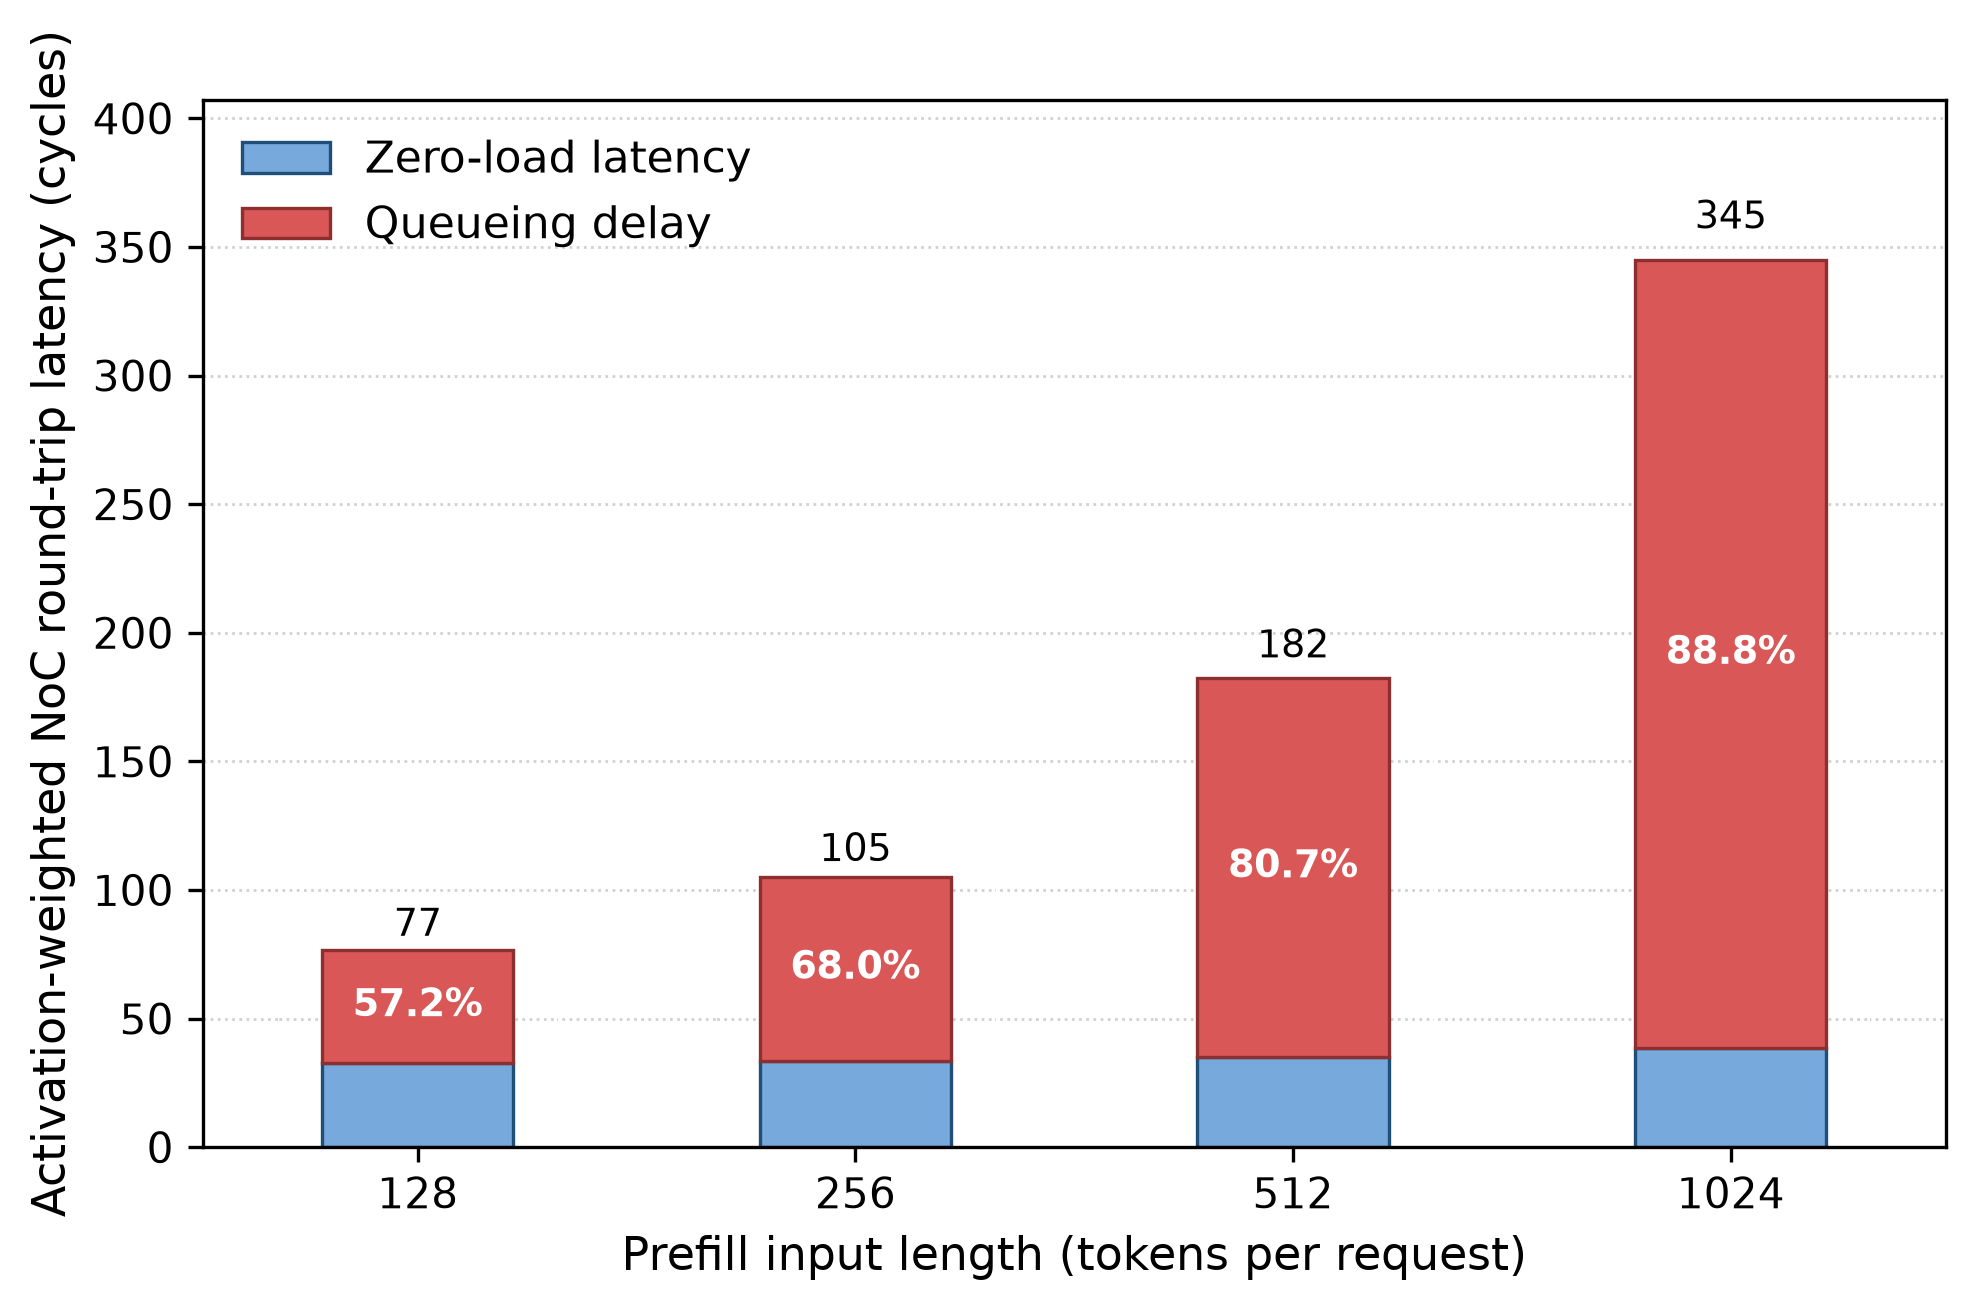
\includegraphics[width=\linewidth]{figures/noc_phenomenon_narrow_bars.png}
  \end{minipage}\hfill
  \begin{minipage}[t]{0.62\columnwidth}
    \vspace{0pt}\centering
    {\fontsize{7}{8}\selectfont\rmfamily\mdseries\upshape (b) Router demand across MoE layers\par}
    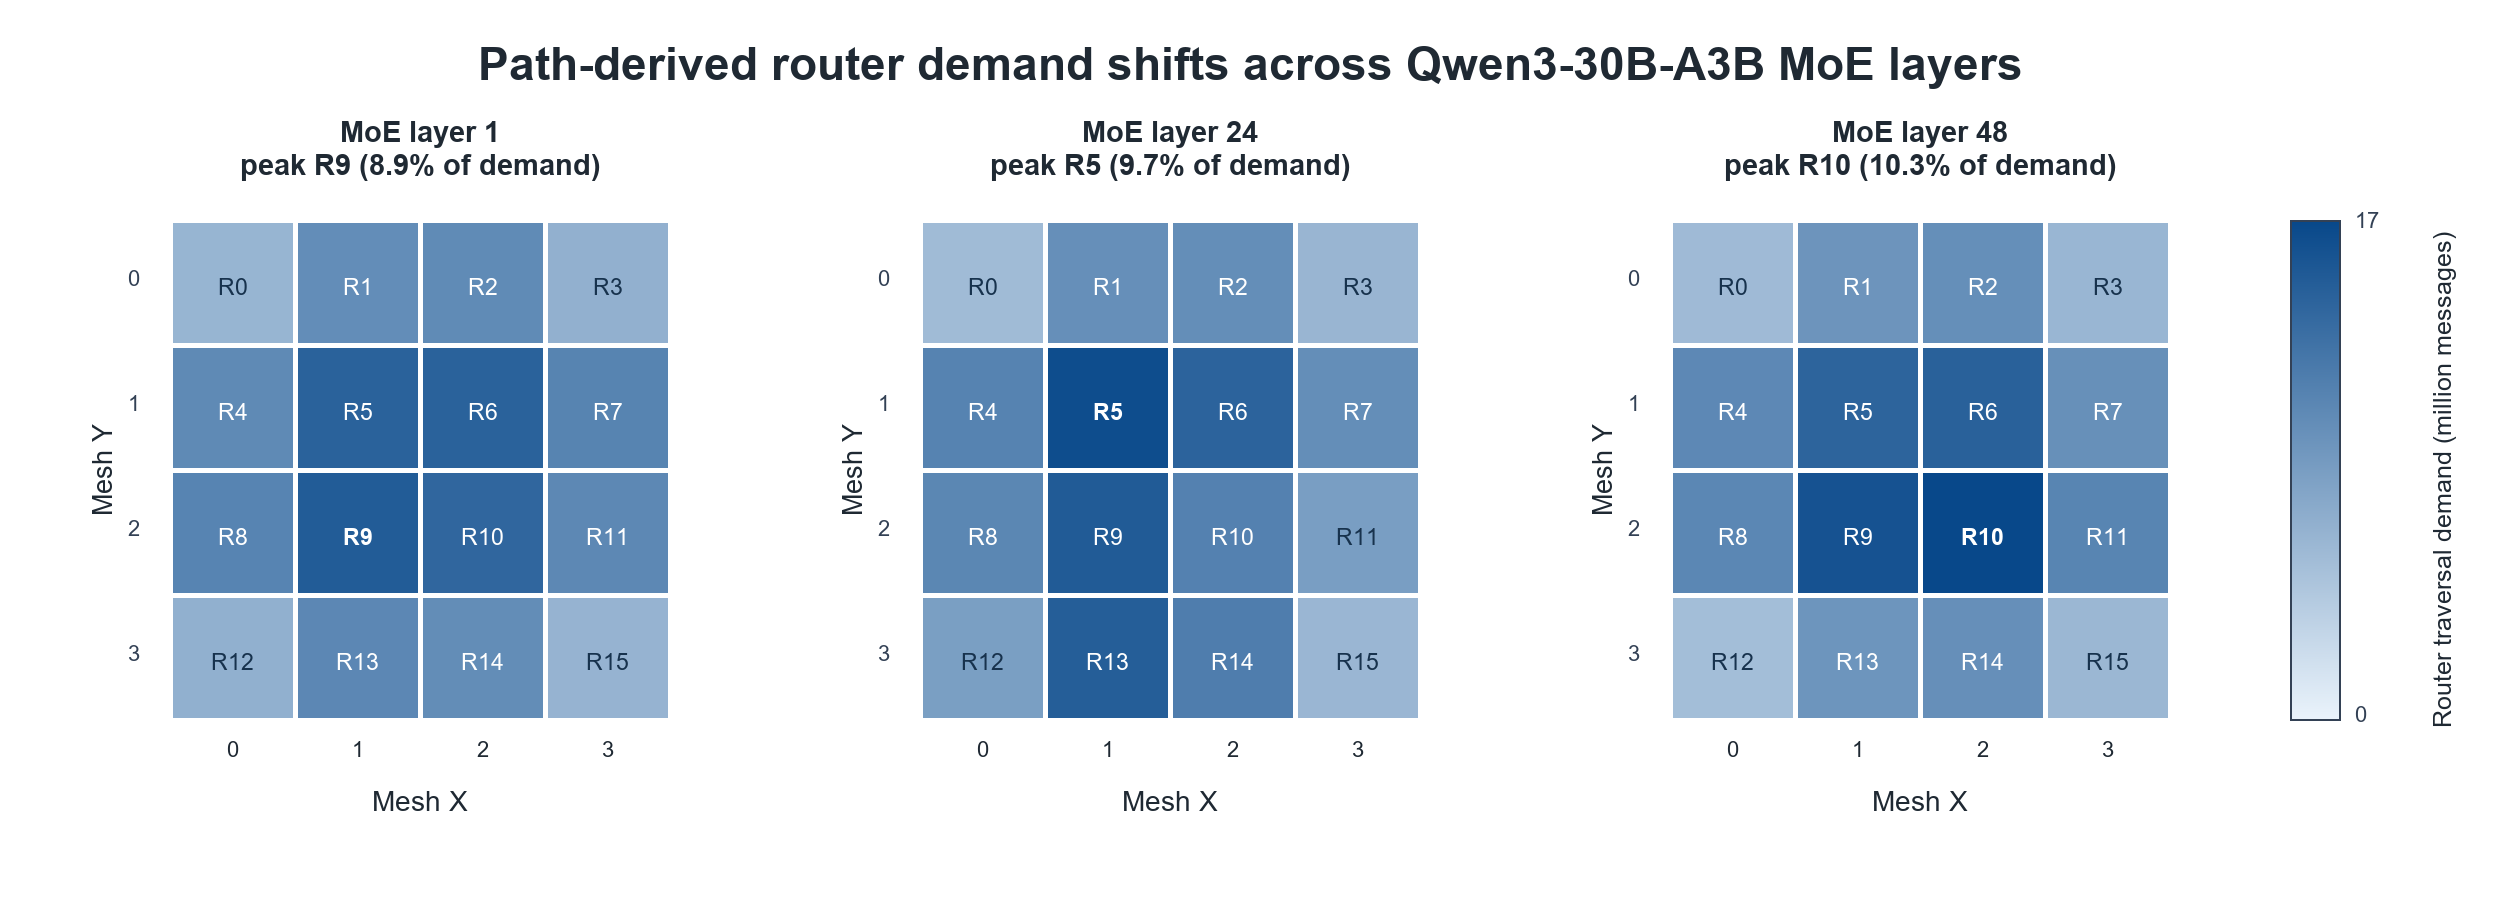
\includegraphics[width=\linewidth,trim=0bp 0bp 0bp 24bp,clip]{figures/noc_cause_router_hotspots_revised.png}
  \end{minipage}
  \caption{Communication latency and router demand for Qwen3-30B-A3B.
  (a) Activation-weighted mean NoC round-trip latency on the fixed Mesh.
  The queueing share rises from 57.2\% to 88.8\% as prefill input grows
  from 128 to 1024 tokens.
  (b) Router demand along deterministic XY paths on a shared color scale.
  The peak moves from R9 to R5 to R10 across MoE layers 1, 24, and 48.}
  \Description{Four stacked bars show the growth in queueing delay with
  input length. Three heatmaps show the change in peak router demand
  across MoE layers.}
  \label{fig:noc-phenomenon}
\end{figure}

\noindent\textbf{Opportunity: Separate Paths for Coherence and MoE.}
Figure~\ref{fig:noc-opportunity}(a) shows a GetS request from $N_0$
and MoE traffic from $N_5$ competing for the $N_4$-to-$N_8$ Mesh
output. Arbitration divides the available link service among these
inputs. A separate coherence Mesh gives GetS requests and their DataS
responses independent physical paths. In
Fig.~\ref{fig:noc-opportunity}(b), they use
$C_0$--$C_4$--$C_8$, while MoE packets remain on plane M.
The network interface (NI) selects the plane by message class and opcode. Both planes
share endpoint memory service.

Within plane M, configurable circuits provide additional paths for
concentrated MoE transfers. The
$\mathrm{NI}_5$--$\mathrm{CS}_3$--$\mathrm{NI}_8$ circuit bypasses
the intermediate Mesh router at $N_4$. Circuits also add channels
between neighboring nodes, while paths through the upper CS network
bypass multiple Mesh routers for distant transfers. These
connections can be reassigned between communication phases as the
busy node pairs change. The circuits share NI service and SRAM-bank
bandwidth.

\begin{figure}[!t]
  \centering
  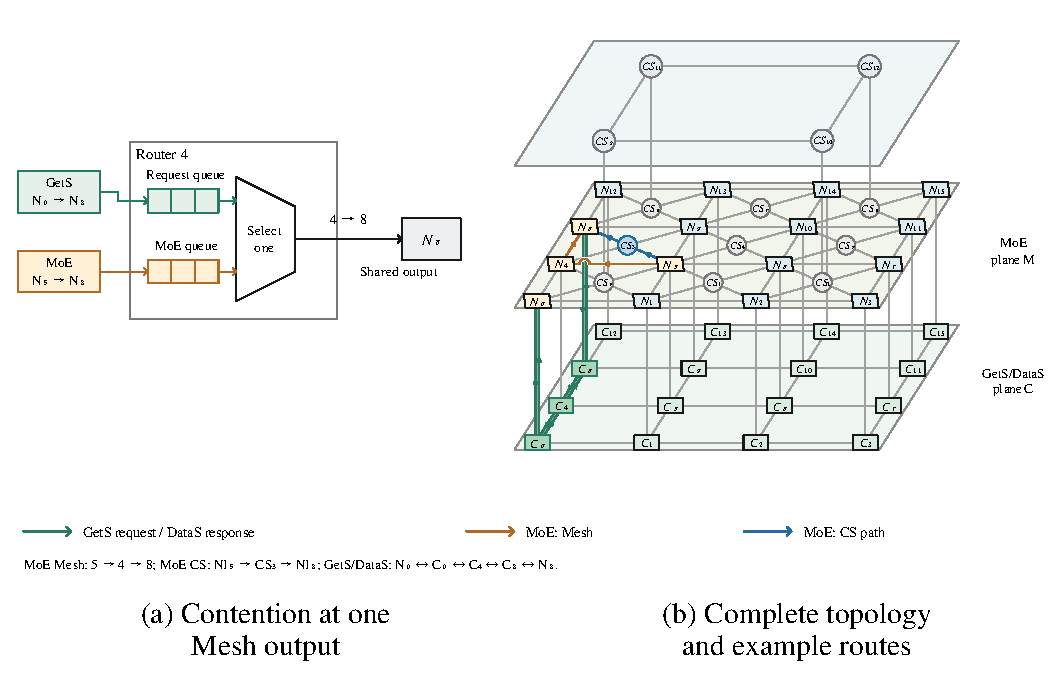
\includegraphics[width=\columnwidth]{figures/noc_opportunity_dual_plane_titles_spaced.pdf}
  \caption{Separate paths for coherence and MoE traffic.
  (a) Two inputs compete for one baseline Mesh output.
  (b) Complete dual-plane topology with GetS/DataS routes and the
  MoE Mesh and CS paths highlighted.}
  \Description{The left panel shows a coherence-request queue and a MoE
  queue sharing the output from node 4 to node 8. The right panel shows
  all sixteen nodes, sixteen coherence routers, thirteen configurable
  switches, and their physical connections.
  Requests and responses traverse C0, C4, and C8; MoE packets use the
  Mesh route or the NI5-CS3-NI8 circuit on plane M.}
  \label{fig:noc-opportunity}
\end{figure}

\noindent\textbf{Thermal Management.}
Concentrated activity in the stacked Logic and DRAM tiers raises temperatures in both tiers, increasing the risk of thermal throttling, which can increase inference latency. While task migration has been widely studied for thermal management, its effectiveness in DRAM-stacked NPUs is limited by the strong dependence of computation on locally stored model weights. Migrating tasks may require weight replication or remote memory accesses, introducing additional DRAM and NoC overhead. Our experiments show that these costs largely offset the performance benefits of task migration. Therefore, instead of relocating tasks, we reduce heat generation through operator-level energy-aware DVFS and improve execution efficiency through thermal-aware task scheduling.

\section{Design}
\label{sec:design}

\subsection{Dual-Plane NoC}
\label{sec:noc-design}

Figure~\ref{fig:noc-physical-design} shows two physically separate
$4\times4$ networks on the logic tier. Plane M carries MoE data and
control messages through the original Mesh and configurable switches
(CSs). Plane C carries GetS shared-read requests and their DataS
responses. Each node $N_i$ connects directly to its corresponding
coherence router $C_i$. The interconnects are routed in the logic die's
metal layers.

The M plane retains nine lower CSs and four upper CSs. Each lower CS
connects to the four corner nodes of a $2\times2$ group. Corner, edge,
and interior nodes thus have one, two, and four CS attachments.
Upper switches $\mathrm{CS}_9$--$\mathrm{CS}_{12}$ form a $2\times2$
network and connect down to $\mathrm{CS}_0$, $\mathrm{CS}_2$,
$\mathrm{CS}_6$, and $\mathrm{CS}_8$, respectively. A local circuit
connects two NIs through one lower CS; a longer circuit uses the upper
network to bypass intermediate Mesh routers. MoE packets use an
assigned circuit or the M-plane Mesh. Coherence requests and responses
use C-plane links independently of these route choices.

\begin{figure}[!t]
  \centering
  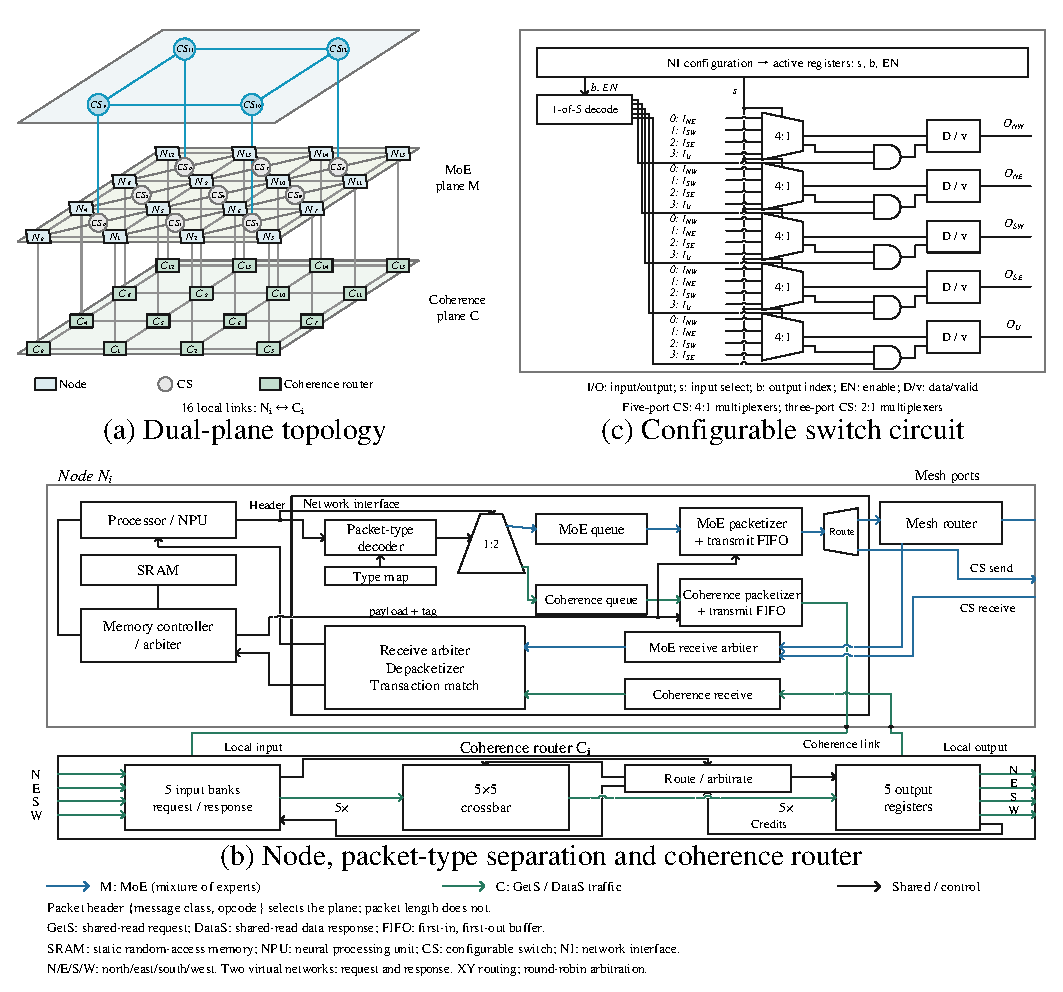
\includegraphics[width=\columnwidth]{figures/noc_dual_plane_uniform_titles.pdf}
  \caption{Dual-plane NoC. (a) MoE Mesh/CS plane M and coherence Mesh
  plane C, with one local connection per node.
  (b) Node, packet-type decoder, and five-port coherence router.
  (c) CS circuit with input selection and output enable.}
  \Description{The upper-left panel shows the two networks and sixteen
  node-to-coherence-router connections. The upper-right panel shows a
  five-direction configurable switch. The lower panel shows packet-type
  classification, separate MoE and coherence queues, packet formation,
  receive processing, shared SRAM arbitration, and the coherence router.}
  \label{fig:noc-physical-design}
\end{figure}

\subsection{Node and Network Interface}
\label{sec:noc-node-design}

Figure~\ref{fig:noc-physical-design}(b) shows an NPU node with banked
SRAM, a network interface (NI), and an M-plane Mesh router. The NI
decodes the message class and opcode before packet formation. Its type
map directs GetS and DataS to plane C and MoE messages to plane M.
A short MoE control message uses M, while a DataS response carrying a
cache line uses C. Separate queues and packetizers feed the two planes;
each packet keeps its selected plane throughout transmission.
Source reads, receive writes, and NPU accesses share the SRAM arbiter.

Each $C_i$ has four neighbor ports and one local NI port, with separate
input queues for requests and responses. These queues form two virtual
networks with independent credits. A $5\times5$ crossbar connects the
input banks to output registers. XY routing selects the next direction,
and round-robin arbitration selects an eligible input. Output registers
hold data until the receiver accepts it. The NI allocates response
storage before issuing GetS; the service endpoint reserves a response
transmit slot before starting the memory operation. Request and response
queues therefore have separate storage and flow-control state.

On plane M, the NI selects the Mesh or a configured CS attachment for
each complete packet. Packets carry a transfer identifier, byte offset,
and transfer length. Receive descriptors supply the destination SRAM
address. The receive arbiter and depacketizer check the packet and
write its payload at that address plus the offset. A receipt bitmap
records accepted writes, and completion is reported when all expected
packet writes finish. Finite receive queues buffer concurrent Mesh
and CS arrivals. The C-plane receive path matches responses to their
request identifiers and shares the endpoint's SRAM write service.

\subsection{Configurable Switches}
\label{sec:noc-switches}

Figure~\ref{fig:noc-physical-design}(c) shows a lower CS with directions
NW, NE, SW, SE, and U. Five four-input multiplexers select among the
other directions' inputs. The configuration fields $s$, $b$, and EN
select the input, output, and connection enable. Output decoding
activates one directed input--output pair. Data and valid propagate
forward, and ready propagates back along the selected connection.
The output register retains its data under backpressure.

Only $\mathrm{CS}_0$, $\mathrm{CS}_2$, $\mathrm{CS}_6$, and
$\mathrm{CS}_8$ have U links. The remaining lower CSs have their U
interfaces disabled. Each upper CS has two neighbor directions and
one downward direction, implemented with three two-input multiplexers.
Separate NI attachments permit concurrent MoE circuits, subject to
shared NI service, direct memory access (DMA) engines, and SRAM bandwidth.

\subsection{Traffic Prediction}
\label{sec:traffic-prediction}

GetS requests and DataS responses use XY routing on plane C. The host
optimizes MoE routes on plane M. For Dispatch, we adapt MixNet's
adjacent-layer predictor~\cite{liao2025mixnet}:
\begin{equation}
  \widehat{\mathbf y}_{\ell,s}=P_\ell\mathbf x_{\ell-1,s},
  \quad P_\ell\geq0,\quad
  \mathbf1^{\mathsf T}P_\ell=\mathbf1^{\mathsf T}.
  \label{eq:noc-load-prediction}
\end{equation}
Here $\mathbf x_{\ell-1,s}$ is the preceding layer's normalized expert distribution
for tokens with known source NI $s$. Weighted least squares fits $P_\ell$
from paired token groups, weighting their size and recency. Prefill and
decode use separate models, with a historical-mean fallback.
Expert placement and packing map forecasts to source--destination
demand. Final allocation uses actual Top-K and packing metadata.
Combine uses confirmed assignments, output shapes, and estimated
expert completion times to derive return packets and release times.

\subsection{Reconfiguration Problem}
\label{sec:noc-problem}

Within a fixed $H$-cycle planning interval, $\mathcal M_f$ contains
the unbound packets of MoE source--destination flow $f$.
Their payloads $b_m$ give $D_f=\sum_{m\in\mathcal M_f}b_m$ and
$\mathcal M=\bigcup_f\mathcal M_f$. Legal CS paths for packet $m$
form $\mathcal P_m$, with $\mathcal P=\bigcup_m\mathcal P_m$.
Each simple path connects the source and destination NI through wired
CS ports. Binary $z_p$ selects path $p$;
binary $x_{m,p}$ assigns packet $m$ to it. We maximize useful payload
assigned to the CS network:
\begin{equation}
  \max_{\mathbf z,\mathbf x}\quad
  V=\sum_{m\in\mathcal M}b_m\sum_{p\in\mathcal P_m}x_{m,p}.
  \label{eq:noc-volume-objective}
\end{equation}
Readiness flag $g_m$ equals one when source data and receive storage
are ready, and zero otherwise. Each packet uses at most one enabled path:
\begin{equation}
  \sum_{p\in\mathcal P_m}x_{m,p}\leq1,
  \qquad x_{m,p}\leq z_p,\quad x_{m,p}\leq g_m.
  \label{eq:noc-packet-assignment}
\end{equation}
Selected paths are CS-disjoint. With $A_{c,p}=1$ when $p$ uses CS $c$,
\begin{equation}
  \sum_{p\in\mathcal P}A_{c,p}z_p\leq1,
  \qquad c=0,\ldots,12.
  \label{eq:noc-cs-exclusion}
\end{equation}

Resource $r\in\mathcal R$ is an M-plane link or NI, DMA, or SRAM service.
Its remaining budget $C_r$ within $H$ deducts work outside $\mathcal M$:
existing transfers, configuration messages, and C-plane use of shared endpoints.
Cost $u_{m,p,r}$ includes framing and expresses service in NoC cycles.
Unassigned packets use the M-plane Mesh, denoted
by 0, with $x_{m,0}=1-\sum_{p\in\mathcal P_m}x_{m,p}$. Thus,
\begin{equation}
  \sum_{m\in\mathcal M}\sum_{p\in\mathcal P_m\cup\{0\}}
  u_{m,p,r}x_{m,p}\leq C_r,\qquad r\in\mathcal R.
  \label{eq:noc-resource-capacity}
\end{equation}
Path $p$ specifies the input, output, and enable fields of each CS;
$x_{m,p}$ determines the source NI's route tag for packet $m$.

\subsection{Configuration Algorithm}
\label{sec:noc-algorithm}

Offline enumeration supplies local and upper-CS paths. At runtime,
flows are sorted by decreasing $D_f$, and packets follow release order.
Each round examines up to $K_f$ largest remaining flows and $K_p$ paths per flow.
An extension adds one or two paths compatible with the selected set
and with each other.
\textsc{Assign} reallocates packets jointly across the full proposed set,
choosing paths by unloaded latency and then identifier. Feasible extensions
enter the candidate pool; the best positive increase in $V$ advances
the search. Ties favor fewer CS changes from the active configuration
$S_0$, then fixed path identifiers. Each successful round occupies a new
CS, giving at most thirteen rounds.

Candidates $S=(\mathbf z,\mathbf x)$ are checked in decreasing $V$.
A timing model propagates
source reads, finite queues, credits, receive writes, and task dependencies.
C responses follow their request's memory service. Both estimates use
the same time origin; $S_0$ continues forwarding during host computation.
For the current phase's required consumers, an update must satisfy
\begin{equation}
  \widehat T(S)+\eta(S)<\widehat T(S_0),
  \label{eq:noc-switching-check}
\end{equation}
where $\eta(S)\geq0$ is calibrated from paired errors on held-out requests.
Protected completion points $k$ additionally satisfy
$\widehat T_k(S)-\widehat T_k(S_0)+\eta_k(S)\leq\epsilon_k$;
they include coherence transactions with specified delay budgets.
Estimates include computation, pause, drain, writes, and NI installation.
After the NI pause acknowledgement, the host refreshes versions and
eligibility and repeats feasibility, timing, and budget checks. Configuration
follows Section~\ref{sec:noc-config-interface}.

\begin{algorithm}[H]
  \caption{MoE-plane CS configuration}
  \label{alg:noc-configuration}
  \small
  \begin{algorithmic}[1]
    \Require MoE packets $\mathcal M$, paths $\mathcal P$, budgets $C_r$, active $S_0$
    \Ensure $S_0$, an acknowledged update, or an update error
    \State Sort flows by $D_f$ and packets by release order
    \State $S\gets$ Mesh allocation; $\mathcal C\gets\varnothing$
    \While{construction budget remains}
      \State Generate compatible one- and two-path extensions
      \State $\mathcal E\gets$ jointly assigned feasible extensions
      \State $\mathcal C\gets\mathcal C\cup\mathcal E$
      \State \textbf{if} no positive added $V$ \textbf{then break}
      \State $S\gets$ extension with largest added $V$
    \EndWhile
    \For{$S'\in\mathcal C$ in decreasing $V$}
      \State \textbf{if} budget expired \textbf{then return} $S_0$
      \State Estimate completion and update overhead
      \If{timing checks pass within the decision budget}
        \State Request packet holds and pause new CS admissions
        \If{pause acknowledged within the decision budget}
          \State Refresh state; recheck feasibility and timing
          \State \textbf{if} final checks pass \textbf{then return} $\Call{ApplyCS}{S'}$
        \EndIf
        \State Release holds and resume $S_0$; \Return $S_0$
      \EndIf
    \EndFor
    \State \Return $S_0$
  \end{algorithmic}
\end{algorithm}


\subsection{Configuration Interface}
\label{sec:noc-config-interface}

The host sends CS configuration commands over the M-plane Mesh.
Each lower CS is configured by its northwest node's NI; that CS relays
commands to its attached upper CS where present. A separate NI
configuration queue feeds the CS command decoder, which writes the
configuration register and returns an acknowledgement. This control
interface is independent of the selected CS data connection.

Table~\ref{tab:noc-command-fields} summarizes the command fields.
A lower CS uses three output-selection bits, two input-selection bits,
and one enable bit; an upper CS uses two, one, and one, respectively.
The output code follows the instance's wired directions, and the input
code indexes that output's allowed inputs. The NI stores each MoE
packet's assigned CS attachment and configuration version in its
transfer descriptor. Unassigned MoE packets use the M-plane Mesh.

\begin{table}[!t]
  \caption{CS configuration command fields.}
  \label{tab:noc-command-fields}
  \centering\small
  \begin{tabularx}{\columnwidth}{@{}p{0.25\columnwidth}>{\raggedright\arraybackslash}X@{}}
    \hline
    Field & Meaning \\
    \hline
    Type & Message class and operation code. \\
    Destination & NI responsible for the target CS. \\
    TransactionID & Command--response matching identifier. \\
    ConfigVersion & CS configuration and matching packet assignments. \\
    Target & CS index or NI transfer descriptor. \\
    Operation & Write, install descriptor, pause, status, or resume. \\
    State & CS input/output selection and enable, or packet assignments. \\
    Status & Success or failure of the requested operation. \\
    \hline
  \end{tabularx}
\end{table}

The NI acknowledges a pause after holding the selected unbound MoE
descriptors and stopping new CS admissions. Admitted transfers retain
their routes. After the final check, \textsc{ApplyCS} drains these
transfers, writes and confirms the CS states, installs matching NI
assignments and versions, and resumes transmission. A rejected final check
releases the holds and resumes $S_0$. A write or installation error
is reported with CS admissions paused until matching CS and NI
configurations are restored. Plane C continues forwarding throughout.

\subsection{Thermal-Aware Execution}
\label{sec:thermal-design}

Thermal-aware execution complements bank placement and
NoC reconfiguration by adjusting operator frequencies and
task start times to reduce latency under thermal constraints.
Let $s_j$ and $r_j$ denote the start time and frequency
ratio of task $j$. The execution objective is
\begin{equation}
\begin{aligned}
  \min_{\{s_j,r_j\}} \quad & T_{\mathrm{inf}} \\
  \mathrm{s.t.}\quad
  & T_b[k]\leq T_{\mathrm{limit}},\quad \forall b,k,
\end{aligned}
\label{eq:thermal-optimization}
\end{equation}
where $T_{\mathrm{inf}}$ is the inference completion time
and $T_b[k]$ is the temperature of physical block $b$ at
thermal sampling step $k$.
We address this objective through offline operator-level
energy-aware DVFS and runtime thermal-aware task scheduling.


\noindent\textbf{Operator-Level Energy-Aware DVFS.}
We profile each operator type at three DVFS settings, $r\in\{1.0,0.75,0.5\}$, with separate profiles for different execution configurations. For each profile, we select the frequency that minimizes total execution energy, including dynamic and idle energy. For operators with overlapping computation and memory accesses, reducing the frequency can lower energy consumption with little increase in execution time. This can reduce heat generation and mitigate thermal throttling during inference.

\noindent\textbf{Model-Based Thermal Scheduling.}
We use a HotSpot-based RC thermal model~\cite{hotspot_tool} to capture delayed heat propagation between the Logic and DRAM tiers. Rather than repeatedly performing full RC simulations during scheduling, we precompute the temperature responses of individual tasks, including delayed temperature peaks after task completion. At runtime, the controller evaluates the predicted temperatures of candidate tasks and selects the task with the earliest feasible start time.

\FloatBarrier

\section{Evaluation Results and Analysis}
\label{sec:experiment}

\subsection{Experimental Setup}
We model a face-to-face hybrid-bonded system with 16 NPU clusters,
32~GiB of HB-DRAM, and a $4\times4$ Mesh with 256-bit links at 1~GHz.
Each cluster has 4096 MACs, a 16-lane vector unit, and 4~MiB SRAM;
each local vertical link provides 25.6~GB/s. Compute, memory, and
thermal model settings are xxx. Table~\ref{tab:eval-workloads} lists
the workloads and measurement boundaries.

\begin{table}[!t]
\caption{Evaluation workloads and measurement boundaries.}
\label{tab:eval-workloads}
\centering\footnotesize
\begin{tabularx}{\columnwidth}{@{}>{\raggedright\arraybackslash}p{0.43\columnwidth}>{\raggedright\arraybackslash}X@{}}
\hline
Workload & Measurement boundary \\
\hline
Qwen3-30B-A3B; Qwen1.5-MoE-A2.7B & Prefill, decode, complete request \\
mini-SWE-agent + Qwen3 & Model calls and Agent task \\
LingBot TI2V & Complete video generation \\
WHISPER + SLAM + $\pi_{0.5}$ & Joint thermal execution \\
\hline
\end{tabularx}
\end{table}

HiBand~\cite{wang2026hiband} is the state-of-the-art comparator.
Both designs use the same inputs, precision, resource budgets, synthetic
coherence request releases, and completion criteria. Input lengths,
concurrency, and mapping are xxx. The fixed Mesh provides an additional
ablation. Each experimental line first records a complete run for calibration.
Subsequent pairs measure the same one or two MoE layers and estimate total
latency using a common dependency model, including non-MoE work and
control costs. We report layer measurements and end-to-end estimates
separately; estimation error is xxx.

We freeze request order, random seeds, and initial memory and thermal
states for each pair. For Agent workloads, we record the completion
of the general-purpose branch, the MoE branch, and the step waiting
for both results. This distinguishes earlier memory responses from
earlier task completion. The synthetic coherence source, transaction
count, and release interval are xxx. Both configurations include the
same request and response dependencies.

\subsection{Performance Comparison}
Figure~\ref{fig:eval-overall} compares completion times with HiBand.
Latency reduction is $1-T_{\mathrm{design}}/T_{\mathrm{HiBand}}$.
Estimated end-to-end latency decreases by xxx\% on average and up to
xxx\%. Language-model time to first token and time per output token
change by xxx\% and xxx\%, respectively. Agent task outcomes and
video-generation completion are checked over the boundaries in
Table~\ref{tab:eval-workloads}; the paired results are xxx.
We also report per-workload reductions and the largest regression,
rather than relying only on an aggregate mean. The fixed-Mesh ablation
uses the same model routes and external arrival schedule to quantify
the effect of the proposed network and bank policies together.

\begin{figure}[!t]
\centering
\fbox{\rule{0pt}{18mm}\rule{0.94\columnwidth}{0pt}}
\caption{Completion times for HiBand, fixed Mesh, and the full design.
Labels distinguish complete-run measurements and end-to-end estimates.}
\Description{Placeholder for paired workload completion times.}
\label{fig:eval-overall}
\end{figure}

\subsection{Ablation and Implementation Overhead}
Figure~\ref{fig:eval-breakdown} traces bank waiting, NoC queueing,
configuration, and consumer readiness on a common timeline.
The fixed-Mesh comparison changes exposed waiting by xxx\%;
the resulting completion-time change is xxx\%.
Thermal ablation retains the same NoC and bank policies and switches
only thermal control. Peak temperature and completion time change by
xxx~$^{\circ}$C and xxx\%, respectively.

\paragraph{Contention and configuration costs.}
Matched traces record source data readiness, packet injection,
router waiting, bank completion, and consumer release. We count
overlapping intervals once when reconstructing the critical path.
Configuration costs include state collection, decision computation,
admission pause, circuit draining, register updates, and transfer
resumption. Comparisons with and without exposed switching costs
yield xxx and xxx; rejected updates and the worst background delay
are xxx. No-overlap and different-output traffic pairs serve as
controls for the shared-output contention mechanism.

\paragraph{Sensitivity.}
We vary coherence request intensity, MoE burst overlap, and
reconfiguration cost under the same resource budget. The corresponding
completion-time changes are xxx. We additionally vary input length
and request concurrency to test whether gains persist as communication
demand changes; the tested ranges and results are xxx. Thermal
experiments report both the initial temperature and the temperature
limit, together with time above the limit and execution progress.
These results distinguish reduced peak temperature from improved
completion time.

\begin{figure}[!t]
\centering
\begin{minipage}{0.47\columnwidth}\centering
\fbox{\rule{0pt}{16mm}\rule{0.88\linewidth}{0pt}}\\
{\fontsize{7}{8}\selectfont\rmfamily\mdseries\upshape (a) Critical-path breakdown}
\end{minipage}\hfill
\begin{minipage}{0.49\columnwidth}\centering
\fbox{\rule{0pt}{16mm}\rule{0.88\linewidth}{0pt}}\\
{\fontsize{7}{8}\selectfont\rmfamily\mdseries\upshape (b) Thermal ablation}
\end{minipage}
\caption{Paired critical-path delays and thermal-control ablation.
Both thermal configurations retain the same NoC and bank policies.}
\Description{Two placeholders for latency breakdown and thermal ablation.}
\label{fig:eval-breakdown}
\label{fig:eval-thermal}
\end{figure}

Table~\ref{tab:eval-cost} compares shared-Mesh and C/M dual-plane cores (two Meshes, 13 CSs), with simplified NIs. Full endpoint, SRAM/bank, distributed-configuration, thermal, and cross-tier hardware is excluded. This RTL differs from the performance-replay implementation; costs and performance are not a matched pair. FPGA: Vivado 2017.4, \texttt{xcku5p-}\allowbreak\texttt{ffva676-2-e}, 200\,MHz OOC post-route static timing. ASIC: Yosys 0.23, Nangate45 TT, common 1\,ns constraints, synthesis area only. Runtime rows count exposed critical-path time.

\begin{table}[!ht]
\caption{Network-core and runtime costs (simplified NIs).}
\label{tab:eval-cost}
\centering\scriptsize
\renewcommand{\arraystretch}{0.85}
\begin{tabularx}{\columnwidth}{@{}>{\raggedright\arraybackslash}Xrr@{}}
\hline
Metric & Shared Mesh & Dual plane + CS \\
\hline
FPGA LUTs / flip-flops & 31,995 / 38,286 & 117,625 / 92,783 \\
FPGA BRAM / DSP & 0 / 0 & 0 / 0 \\
FPGA setup WNS (ns), 200\,MHz & $+0.339$ & $+0.043$ \\
ASIC synthesis area (mm$^2$) & 0.332176 & 0.869972 \\
ASIC area increase (\%) & --- & 161.90 \\
\hline
Exposed decision overhead (\%) & xxx & xxx \\
Exposed configuration delay (\%) & xxx & xxx \\
\hline
\end{tabularx}
\end{table}

\FloatBarrier

\section{Related Works}
\label{sec:related-works}

\paragraph{Reconfigurable NoCs and traffic management}
SMART~\cite{krishna2013smart} enables packets to bypass multiple routers
within a cycle, reducing traversal latency. HiBand~\cite{wang2026hiband}
reallocates local and global bandwidth through four NoC modes for
HB-DRAM inference. Application-aware prioritization~\cite{das2009priority}
ranks packets according to their applications' stall-time criticality.
These studies address traversal cost, bandwidth allocation, and
shared-resource arbitration. Our design combines separate coherence and
MoE planes with configurable MoE circuits, selecting connections according
to communication demand and checking their effect on consumer completion time.

\paragraph{MoE communication and memory optimization}
ExpertFlow~\cite{he2026expertflow} combines routing prediction, token
scheduling, and expert caching to reduce parameter transfers during
memory-constrained inference. MixNet~\cite{liao2025mixnet} adapts an
optical-electrical fabric to changing expert communication demands in
distributed MoE training. HBSpec~\cite{wang2026hbspec} uses
communication-aware mapping and operator scheduling for hybrid-bonded
speculative decoding. Together, these studies demonstrate the importance
of coordinating computation and data movement. Our work applies demand
prediction to on-chip circuit allocation and accounts for network interface
capacity, memory bank access, and reconfiguration overhead when evaluating
concurrent general-purpose tasks and MoE inference.

\paragraph{Thermal management in 3D systems}
Tasa~\cite{he2025tasa} addresses thermal constraints in 3D-stacked LLM
systems through cross-stack thermal optimization and bandwidth sharing.
Thermal-aware scheduling has also been studied for controlling runtime
temperature in 3D multicore processors~\cite{tsai2016thermal}.
Our thermal mechanism combines operator-level energy-aware DVFS with
scheduling based on predicted temperature responses. It accounts for
delayed heat propagation between logic and DRAM tiers and evaluates
thermal control with the same NoC and bank policies enabled in both
configurations.

\noindent\begin{minipage}{\columnwidth}
\section{Conclusion}
\label{sec:conclusion}

We presented thermal-aware NoC reconfiguration for concurrent
general-purpose computing and MoE inference in 3D-stacked systems.
Separate traffic planes and configurable MoE circuits adapt communication
paths to changing demand. A completion-time check accounts for memory
access and reconfiguration costs, while operator-level DVFS and
thermal-aware scheduling manage execution under temperature constraints.
Compared with HiBand, the design reduces estimated end-to-end latency by
xxx\% on average and up to xxx\%. Thermal control reduces peak temperature
by xxx~$^{\circ}$C, with an execution-time change of xxx\%.

\end{minipage}

\clearpage
\balance
\bibliographystyle{IEEEtran}
\bibliography{references,thermal_references}

\end{document}

